\chapter{¿Qué es la respiración?}\label{ch:g7:what-is-respiration}

Mete una cochinilla en un tarro cerrado y, unas horas después, el aire
del tarro ha cambiado: ha desaparecido parte de su \omterm{def:g7:what-is-respiration:respiration}{oxígeno}, sustituido
por \omterm{def:g7:what-is-respiration:respiration}{dióxido de carbono}. Repítelo con una \omterm{def:g2:from-seed-to-plant:seed}{semilla} que \omterm{def:g2:from-seed-to-plant:germination}{germina}, una seta,
un \omterm{prop:g3:sorting-living-things:groups}{pez} de colores o una cucharada de \omterm{def:g6:decomposers-and-soil:soil}{suelo} vivo --- el mismo resultado,
todas las veces. La \cref{prop:g4:breathing:exchange} enseñó el
intercambio en tu propio pecho; este curso abre la idea a todo su
ancho: el intercambio no es una costumbre humana, sino una propiedad de
la vida misma.

\section{La respiración, definida y medida}

\begin{definition}[Respiración]\label{def:g7:what-is-respiration:respiration}
La \emph{respiración}\index{respiración} es el intercambio de gases por
el que un \omterm{def:g6:exploring-our-environment:components}{ser vivo} toma \emph{oxígeno}\index{oxígeno} de su \omterm{def:g6:exploring-our-environment:components}{entorno} y
suelta \emph{dióxido de carbono}\index{dióxido de carbono}. No hay que
confundirla con la \emph{ventilación}\index{ventilación} --- los
movimientos visibles del pecho de la
\cref{def:g4:breathing:movements}: la ventilación es una manera de
\emph{servir} a la respiración; la respiración misma es el intercambio
de gases, y ocurre en todas las \omterm{def:g5:first-look-at-cells:cell}{células} vivas, haya movimientos o no.
\end{definition}

\begin{proposition}[Cómo se demuestra el intercambio]\label{prop:g7:what-is-respiration:shown}
Dos pruebas de laboratorio corrientes revelan la \omterm{def:g7:what-is-respiration:respiration}{respiración}:
\begin{itemize}
  \item una \emph{sonda de \omterm{def:g7:what-is-respiration:respiration}{oxígeno}} en un recipiente cerrado enseña
        cómo baja el nivel de \omterm{def:g7:what-is-respiration:respiration}{oxígeno} mientras dentro hay un \omterm{def:g6:exploring-our-environment:components}{ser vivo};
  \item el \emph{agua de cal}\index{agua de cal}, un líquido
        transparente que se vuelve lechoso con \omterm{def:g7:what-is-respiration:respiration}{dióxido de carbono}, se
        enturbia cuando se hace pasar por ella el aire del recipiente.
\end{itemize}
\omterm{def:g7:what-is-respiration:respiration}{Oxígeno} que baja y \omterm{prop:g7:what-is-respiration:shown}{agua de cal} que se enturbia, con un recipiente
testigo sin vida que no cambia
(\cref{met:g4:what-plants-need:fairtest} --- la prueba justa nos sigue
a todas partes): eso es la \omterm{def:g7:what-is-respiration:respiration}{respiración}, medida.
\end{proposition}
\admitted

\begin{example}[La galería de los que respiran]\label{ex:g7:what-is-respiration:gallery}
Pásale las dos pruebas a una colección: un ratón --- caída rápida,
enturbiamiento veloz; una cochinilla --- lo mismo, más pequeño; un
guisante que \omterm{def:g2:from-seed-to-plant:germination}{germina} --- inconfundible (un tarro de guisantes brotando
puede agotar su \omterm{def:g7:what-is-respiration:respiration}{oxígeno} en un día); una seta --- sí; caracoles de
charca --- sí; una cucharada de \omterm{def:g6:decomposers-and-soil:soil}{suelo} vivo --- sí, con sus miles de
millones de \omterm{def:g6:decomposers-and-soil:decomposers}{descomponedores} respirando a la vez
(\cref{ex:g6:decomposers-and-soil:handful}). Solo el tarro testigo ---
guijarros, arena seca --- no cambia nada.
\end{example}

\begin{omfigure}
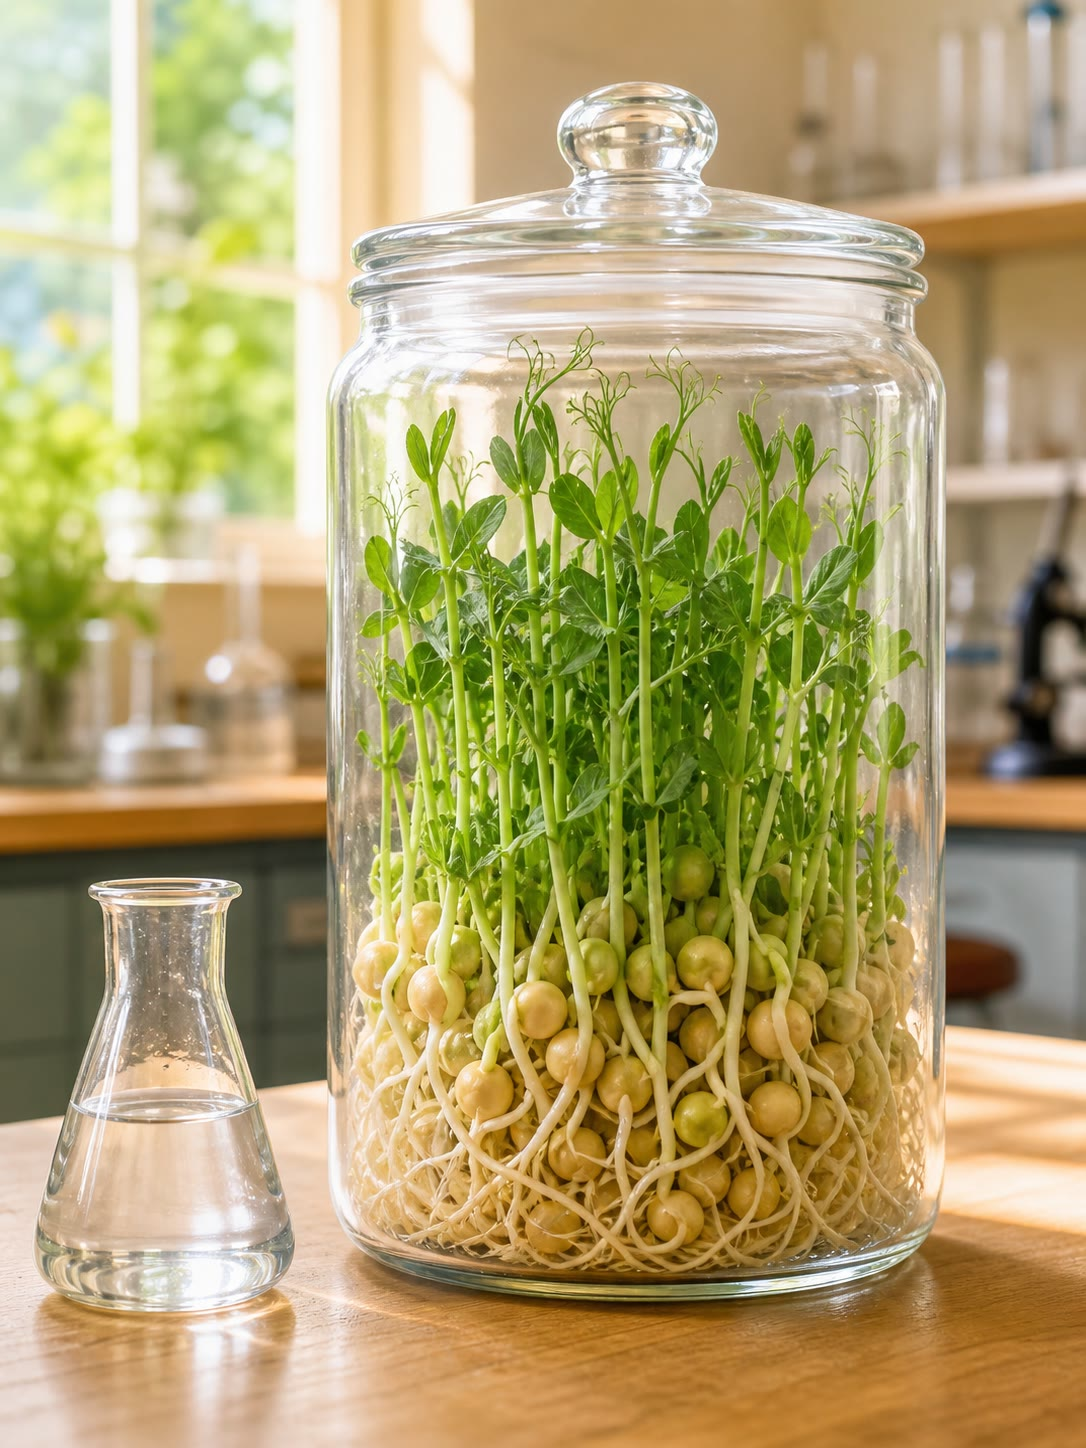
\includegraphics[width=0.46\linewidth]{images/book1/ai/g7-resp-peajar.jpg}

{\small El que respira con más discreción de todo el laboratorio: un
tarro de guisantes brotando puede agotar su \omterm{def:g7:what-is-respiration:respiration}{oxígeno} en un día.}
\end{omfigure}

\begin{remark}[Las plantas también respiran]\label{rem:g7:what-is-respiration:plants}
La \cref{rem:g6:plants-are-producers:gas} ya lo dijo de pasada; el
tarro lo demuestra: una \omterm{def:g1:plants-around-us:plant}{planta} en maceta \emph{a oscuras} baja el
\omterm{def:g7:what-is-respiration:respiration}{oxígeno} de su tarro y enturbia el \omterm{prop:g7:what-is-respiration:shown}{agua de cal} igual que cualquier
\omterm{def:g1:animals-around-us:animal}{animal}. A la \omterm{def:g6:exploring-our-environment:conditions}{luz} del día, la fabricación de las \omterm{def:g5:food-webs:roles}{productoras} enmascara
el efecto --- porque toma mucho más \omterm{def:g7:what-is-respiration:respiration}{dióxido de carbono} del que suelta
la \omterm{def:g7:what-is-respiration:respiration}{respiración} --- pero la \omterm{def:g7:what-is-respiration:respiration}{respiración} no se para nunca. Ser verde no
excusa a una \omterm{def:g5:first-look-at-cells:cell}{célula} de respirar en sentido amplio; no hay nada vivo
excusado.
\end{remark}

\section{Por qué respiran los seres vivos}

\begin{proposition}[La respiración da fuerza a las células]\label{prop:g7:what-is-respiration:power}
El sentido del intercambio es la \emph{\omterm{prop:g3:balanced-diet:jobs}{energía}}. En todas las \omterm{def:g5:first-look-at-cells:cell}{células}
vivas, los \omterm{def:g4:journey-of-food:digestion}{nutrientes} (\cref{def:g4:journey-of-food:digestion}) se
\emph{queman} despacio con el \omterm{def:g7:what-is-respiration:respiration}{oxígeno} que trae la \omterm{def:g7:what-is-respiration:respiration}{respiración}: su
\omterm{prop:g3:balanced-diet:jobs}{energía} se libera para el trabajo de la \omterm{def:g5:first-look-at-cells:cell}{célula} --- \omterm{def:g3:bones-and-muscles:muscle}{contraerse},
construir, mandar --- y el \omterm{def:g7:what-is-respiration:respiration}{dióxido de carbono} es el resto quemado, que
se retira. La ``parte quemada'' de la
\cref{prop:g6:matter-from-food:losses} era exactamente esto, vista
desde la contabilidad; aquí se ve desde la \omterm{def:g5:first-look-at-cells:cell}{célula}.
\end{proposition}
\admitted

\begin{example}[La comparación con el fuego, usada con honradez]\label{ex:g7:what-is-respiration:fire}
La llama de una vela también consume \omterm{def:g7:what-is-respiration:respiration}{oxígeno} y suelta \omterm{def:g7:what-is-respiration:respiration}{dióxido de
carbono} --- arder y respirar son de verdad la misma clase de química.
Las diferencias importan igual: la quema de la \omterm{def:g5:first-look-at-cells:cell}{célula} es lenta, sin
llama, repartida en miles de pasos diminutos, y su \omterm{prop:g3:balanced-diet:jobs}{energía} se captura
para trabajar en vez de perderse en \omterm{def:g6:exploring-our-environment:conditions}{luz} y chamusquina. La \omterm{def:g7:what-is-respiration:respiration}{respiración}
es combustión domesticada --- fuego con correa, en todas tus \omterm{def:g5:first-look-at-cells:cell}{células}.
\end{example}

\begin{example}[Leer la demanda]\label{ex:g7:what-is-respiration:demand}
Como la quema paga el trabajo, la demanda sigue al esfuerzo: el niño
que esprinta del \cref{ex:g4:breathing:running} respira mucho más
deprisa que quien lee en el sillón; el guisante que \omterm{def:g2:from-seed-to-plant:germination}{germina} ---
construyendo una \omterm{def:g1:plants-around-us:plant}{planta} a toda velocidad
(\cref{def:g2:from-seed-to-plant:germination}) --- respira mucho más
deprisa que la \omterm{def:g2:from-seed-to-plant:seed}{semilla} seca que espera a su lado, cuya \omterm{def:g7:what-is-respiration:respiration}{respiración} está
al ralentí durante años. La \omterm{def:g7:what-is-respiration:respiration}{respiración} es el ruido del motor de la
vida: fuerte en el esfuerzo y en el crecimiento, un susurro en el
letargo y silencio solo en la muerte.
\end{example}

\section{La respiración en todos los hábitats}

\begin{proposition}[Una misma necesidad, muchos entornos]\label{prop:g7:what-is-respiration:habitats}
Todos los \omterm{def:g6:exploring-our-environment:components}{seres vivos} tienen que conseguir su \omterm{def:g7:what-is-respiration:respiration}{oxígeno} \emph{de su
\omterm{def:g6:exploring-our-environment:components}{entorno}} --- y los \omterm{def:g6:exploring-our-environment:components}{entornos} son distintos. El aire es rico en \omterm{def:g7:what-is-respiration:respiration}{oxígeno};
el agua tiene mucho menos, disuelto (el \cref{exo:g4:breathing:11} se
encontró con la consecuencia); el \omterm{def:g6:decomposers-and-soil:soil}{suelo} y el barro tienen todavía
menos. Dónde y cómo vive un \omterm{def:g6:exploring-our-environment:components}{ser vivo} lo moldea, por tanto, la manera en
que resuelve su problema de \omterm{def:g7:what-is-respiration:respiration}{oxígeno} --- el tema de los dos capítulos
siguientes, para el equipo de los \omterm{def:g1:animals-around-us:animal}{animales}
(\cref{ch:g7:how-animals-breathe}) y para la economía del agua
(\cref{ch:g7:oxygen-in-the-water}).
\end{proposition}
\admitted

\begin{method}[Poner a prueba una pregunta sobre la respiración]\label{met:g7:what-is-respiration:test}
Para poner a prueba cualquier afirmación sobre la \omterm{def:g7:what-is-respiration:respiration}{respiración} (``las
\omterm{prop:g3:flowers-fruits-seeds:transform}{semillas} respiran más deprisa con calor'', ``el barro de la charca
respira''):
\begin{enumerate}
  \item encierra al sujeto en un recipiente, con una sonda de \omterm{def:g7:what-is-respiration:respiration}{oxígeno} o
        con una trampa de \omterm{prop:g7:what-is-respiration:shown}{agua de cal};
  \item monta el testigo gemelo --- el mismo recipiente, con el sujeto
        ausente o sin vida;
  \item varía una sola condición cada vez, si la afirmación nombra
        alguna (calor, \omterm{def:g6:exploring-our-environment:conditions}{humedad}, oscuridad);
  \item lee el veredicto en la diferencia: \omterm{def:g7:what-is-respiration:respiration}{oxígeno} bajado, \omterm{prop:g7:what-is-respiration:shown}{agua de cal}
        enturbiada --- frente a la quietud del testigo.
\end{enumerate}
\end{method}

\begin{example}[El método con una semilla fría]\label{ex:g7:what-is-respiration:coldseed}
Afirmación: los guisantes que germinan respiran más despacio con frío.
Dos tarros de guisantes brotando, uno a \omterm{def:g6:exploring-our-environment:conditions}{temperatura} ambiente y otro en
la nevera; trampas de \omterm{prop:g7:what-is-respiration:shown}{agua de cal} en los dos; y un tercero sin vida
como testigo. Al día siguiente: el \omterm{prop:g7:what-is-respiration:shown}{agua de cal} del tarro caliente está
lechosa, la del frío apenas empañada y la del testigo transparente.
Veredicto: la \omterm{def:g7:what-is-respiration:respiration}{respiración} va al ritmo de trabajo de los guisantes ---
la regla de las \omterm{def:g6:exploring-our-environment:conditions}{condiciones} de la
\cref{prop:g6:decomposers-and-soil:speed}, medida en gases.
\end{example}

\section{Ejercicios}

\begin{exercise}[$\star$]\label{exo:g7:what-is-respiration:1}
Define la \omterm{def:g7:what-is-respiration:respiration}{respiración} y distínguela de la \omterm{def:g7:what-is-respiration:respiration}{ventilación}.
\end{exercise}

\begin{exercise}[$\star$]\label{exo:g7:what-is-respiration:2}
Nombra las dos pruebas de laboratorio que revelan la \omterm{def:g7:what-is-respiration:respiration}{respiración} y qué
enseña cada una.
\end{exercise}

\begin{exercise}[$\star$]\label{exo:g7:what-is-respiration:3}
¿Por qué necesita todo experimento de \omterm{def:g7:what-is-respiration:respiration}{respiración} un recipiente testigo
sin vida?
\end{exercise}

\begin{exercise}[$\star$]\label{exo:g7:what-is-respiration:4}
¿Cuál es el sentido de la \omterm{def:g7:what-is-respiration:respiration}{respiración}, según la
\cref{prop:g7:what-is-respiration:power}? ¿Qué es el \omterm{def:g7:what-is-respiration:respiration}{dióxido de carbono}
en esa explicación?
\end{exercise}

\begin{exercise}[$\star$]\label{exo:g7:what-is-respiration:5}
Enumera cinco \omterm{def:g6:exploring-our-environment:components}{seres vivos} muy distintos a los que el
\cref{ex:g7:what-is-respiration:gallery} enseña respirando.
\end{exercise}

\begin{exercise}[$\star$]\label{exo:g7:what-is-respiration:6}
¿Cómo se puede demostrar que una \omterm{def:g1:plants-around-us:plant}{planta} respira, si la \omterm{def:g6:exploring-our-environment:conditions}{luz} del día
enmascara el efecto?
\end{exercise}

\begin{exercise}[$\star\star$]\label{exo:g7:what-is-respiration:7}
Da dos parecidos honrados y dos diferencias honradas entre la quema de
una vela y la \omterm{def:g7:what-is-respiration:respiration}{respiración} de una \omterm{def:g5:first-look-at-cells:cell}{célula}.
\end{exercise}

\begin{exercise}[$\star\star$]\label{exo:g7:what-is-respiration:8}
Ordena por ritmo de \omterm{def:g7:what-is-respiration:respiration}{respiración}, con razones: un guisante seco, un
guisante que \omterm{def:g2:from-seed-to-plant:germination}{germina}, un niño que esprinta, un niño que lee.
\end{exercise}

\begin{exercise}[$\star\star$]\label{exo:g7:what-is-respiration:9}
Un tarro sellado de guisantes brotando pasa la noche; a la mañana
siguiente, una vela que se baja dentro se apaga en el acto. Explícalo
con este capítulo --- y di qué habría enseñado mientras tanto la trampa
de \omterm{prop:g7:what-is-respiration:shown}{agua de cal}.
\end{exercise}

\begin{exercise}[$\star\star$]\label{exo:g7:what-is-respiration:10}
Diseña, con el \cref{met:g7:what-is-respiration:test}, el experimento
para: ``el \omterm{def:g6:decomposers-and-soil:soil}{suelo} vivo respira; el \omterm{def:g6:decomposers-and-soil:soil}{suelo} horneado y sin vida no''.
\end{exercise}

\begin{exercise}[$\star\star$]\label{exo:g7:what-is-respiration:11}
¿Por qué le dan miedo a quien lleva un almacén de grano los montones de
grano húmedo que se calientan solos? Relaciona el
\cref{ex:g7:what-is-respiration:demand} con el calor del montón de
compost (\cref{ex:g6:decomposers-and-soil:compost}).
\end{exercise}

\begin{exercise}[$\star\star\star$]\label{exo:g7:what-is-respiration:12}
``La \omterm{def:g7:what-is-respiration:respiration}{ventilación} es un comportamiento; la \omterm{def:g7:what-is-respiration:respiration}{respiración} es química; la
primera sirve a la segunda''. Defiende cada parte con una observación
de este capítulo o del \cref{ch:g4:breathing}.
\end{exercise}

\section{Problema: Los tarros sellados}

\begin{problem}[{Problema de fin de semana --- seis tarros, dos
misterios y un intercambio de gases}]\label{pb:g7:what-is-respiration:1}
Para la feria de ciencias, la clase prepara seis tarros sellados, cada
uno con una sonda de \omterm{def:g7:what-is-respiration:respiration}{oxígeno} y una trampa de \omterm{prop:g7:what-is-respiration:shown}{agua de cal}: A ---
guijarros; B --- guisantes secos; C --- guisantes que germinan; D ---
un ratón (con comida, agua y solo unas horas, bajo la vigilancia del
profesor); E --- una \omterm{def:g1:plants-around-us:plant}{planta} verde a la \omterm{def:g6:exploring-our-environment:conditions}{luz}; F --- una \omterm{def:g1:plants-around-us:plant}{planta} igual
dentro de una caja oscura.

\medskip\noindent\textbf{Parte I --- Predicciones.}
\begin{enumerate}
  \item Predice las lecturas de A y di cuál es el papel de A en el
        experimento.
  \item Predice B y C, y explica la diferencia aunque los dos tarros
        lleven ``los mismos'' guisantes.
  \item Predice D y di por qué el profesor limita las horas.
  \item E y F llevan \omterm{def:g1:plants-around-us:plant}{plantas} idénticas. Predice la tendencia del
        \omterm{def:g7:what-is-respiration:respiration}{oxígeno} de cada tarro y reconcilia la diferencia con la
        \cref{rem:g7:what-is-respiration:plants}.
\end{enumerate}

\medskip\noindent\textbf{Parte II --- Resultados y lecturas.}
\begin{enumerate}[resume]
  \item Los datos de la mañana coinciden con las predicciones --- solo
        que un compañero se asombra de que la \omterm{def:g1:plants-around-us:plant}{planta} de F ``respire
        como un \omterm{def:g1:animals-around-us:animal}{animal}''. Expón qué enseña F en realidad y qué esconde E.
  \item El \omterm{def:g7:what-is-respiration:respiration}{oxígeno} de C bajó tres veces más deprisa que el de B por
        gramo de guisantes. Traduce ese factor tres a los términos del
        \cref{ex:g7:what-is-respiration:demand}.
  \item El \omterm{prop:g7:what-is-respiration:shown}{agua de cal} de D fue la que se enturbió más deprisa de
        todas. Da la cadena --- del cuerpo caliente y en movimiento del
        ratón hasta el líquido lechoso --- en cuatro pasos.
  \item Nombra la única conclusión que apoyan B, C, D y F a la vez, en
        una frase que empiece por ``Todos los \omterm{def:g6:exploring-our-environment:components}{seres vivos}\dots''.
\end{enumerate}

\medskip\noindent\textbf{Parte III --- Apretar un poco más.}
\begin{enumerate}[resume]
  \item Se propone un séptimo tarro: rodajas de seta. Predice sus
        lecturas y di qué punto de nivel de reino del
        \cref{ex:g7:what-is-respiration:gallery} añadiría.
  \item Los visitantes de la feria preguntan por qué le importa el
        tarro C a los agricultores. Responde con el almacén de grano
        del \cref{exo:g7:what-is-respiration:11}.
  \item Un octavo tarro: agua de charca con su barro. El \omterm{def:g7:what-is-respiration:respiration}{oxígeno} baja
        de la noche a la mañana. ¿Quién respira dentro del tarro y por
        qué importa el hallazgo para la pregunta del
        \cref{ch:g7:oxygen-in-the-water}?
  \item Cierra el cartel de la feria con la distinción del capítulo:
        ¿qué tarros enseñaron \emph{\omterm{def:g7:what-is-respiration:respiration}{ventilación}} y cuáles enseñaron
        \emph{\omterm{def:g7:what-is-respiration:respiration}{respiración}}? (Cuidado --- una de las dos palabras los
        cubre a todos.)
\end{enumerate}
\end{problem}
